\documentclass[ukrainian,14pt]{extarticle}
%\documentclass[14pt]{
\usepackage{chngcntr}

\counterwithin*{equation}{section}
% \counterwithin*{equation}{subsection}

\usepackage{babel}
\usepackage[utf8]{inputenc}
\usepackage{fullpage}
\usepackage{breqn}
\usepackage{ upgreek }
\usepackage{amsmath}
\usepackage{pifont}
\usepackage[bookmarks=true]{hyperref}
\usepackage{bookmark}
\usepackage{graphicx}
\usepackage{tocloft}
\usepackage{listings}
\usepackage{indentfirst}

\usepackage{listings}
\usepackage{color}
 
\definecolor{codegreen}{rgb}{0,0.6,0}
\definecolor{codegray}{rgb}{0.5,0.5,0.5}
\definecolor{codepurple}{rgb}{0.58,0,0.82}
\definecolor{backcolour}{rgb}{0.95,0.95,0.92}
 
\lstdefinestyle{mystyle}{
    backgroundcolor=\color{backcolour},   
    commentstyle=\color{codegreen},
    keywordstyle=\color{magenta},
    numberstyle=\tiny\color{codegray},
    stringstyle=\color{codepurple},
    basicstyle=\footnotesize,
    breakatwhitespace=false,         
    breaklines=true,                 
    captionpos=b,                    
    keepspaces=true,                 
    numbers=left,                    
    numbersep=5pt,                  
    showspaces=false,                
    showstringspaces=false,
    showtabs=false,                  
    tabsize=2
}
 
\lstset{style=mystyle}




\renewcommand\cftsecleader{\cftdotfill{\cftdotsep}}

\def\ab{[a,b]}
\newcommand{\sign}{\operatorname{sign}}

\begin{document}

%\newpage
%\tableofcontents
\newpage

%%%%%%%%%%%%%%%%%%%%%%%%%%%%%%%%%%%%%%%%%
%%%
%%%  Розділ 1.1 Скорочення Пізюра Я.В.
%%%
%%%%%%%%%%%%%%%%%%%%%%%%%%%%%%%%%%%%%%%%%

Необхідність моделювання функціональних залежностей виникає в багатьох галузях прикладної математики та інформатики. При розв’язуваннi багатьох задач науково-технiчного характеру доводиться використовувати функції задані таблицею. Проте часто необхідно мати значення функції в точках, яких немає в таблиці. Також виникає необхідність використання простої функції замість складної.

Найменшу похибку наближення дає мінімаксне (чебишовське) наближення. Особливістю моделей, які побудовані на основі мінімаксного наближення, є те, що вони забезпечують найменшу із можливих похибку апроксимації при заданій кількості параметрів. Саме це зумовлює їхню практичну цінність в отриманні розв’язків задач, для яких важлива висока точність відтворення функціональної залежності [3,11]. До знаходження мінімаксного наближення зводиться розв’язування багатьох наукових та інженерних задач, так як воно значно переважає інші види наближень серед застосувань різних способів наближення функцій [23]. Проте використання на практиці мінімаксного наближення часто не є зручним, бо через обчислювальну похибку неможливо досягнути заданої точності. Цього недоліку не мають наближення сплайнами. Параметри класичних сплайнів використовують, в основному, для узгодження значень функцій і похідних в точках стику. Вони легко обчислюються на комп'ютері і за останній час отримали широке розповсюдження в багатьох областях математики.

Використаня таких сплайнів для наближення аналітичних або таблично заданих функцій може бути не зручним у зв'язку з тим що при цьому необхідно зберігати багато параметрів наближень. В багатьох технічних задачах неперервність похідних наближуючих виразів не потрібне. При побудові цифрових функціональних перетворень часто не потрібно навіть неперервності наближаючих виразів. В таких випадках природньо використовувати для наближеннях виразу - рівномірні сплайни, тобто наближення за допомогою відрізків мінімаксних рівномірних наближень або мінімаксних рівномірних наближень з зафіксованими границями. Властивості рівномірних сплайнів різних видів і алгоритми знаходження їхніх параметрів розглянуті в роботах [9, 15-19, 27, 31 - 34, 39].
Метою моєї магістерської роботи є застосування мінімаксних многочленних наближень, сплайнів мінімаксних многочленних наближень для моделювання функціональних залежностей.

У першому розділі наведено основні поняття та алгоритми для побудови рівномірних наближень чебишовськими сплайнами.
Другий розділ присвячений точності апроксимації многочленими чебишовськими сплайнами.
У третьому розділі описано програму, яка здійснює побудову мінімаксних многочленних наближень сплайнами та наближень з заданою кількістю ланок.
У висновках містяться висновки, отримані в результаті виконання магістерської кваліфікаційної роботи. У додатках містяться текст програми та скріншоти основних результатів роботи програми.

\newpage

\section{Побудова рівномірних наближень чебишовськими сплайнами}
\subsection{Побудова чебишовського многочленного наближення}
За теоремою Вейєрштрасса [1,21] довільну неперервну функцію $f(x)$  можна наблизити многочленом $P_m(x)$ із будь-якою точністю $\epsilon$. Серед усіх способів наближення функцій найменшу похибку дає найкраще чебишовське (мінімаксне) наближення [16]. Найкращим чебишовським зваженим наближенням називають вираз $F(A, x) \in F(B, x)$, для якого максимум модуля зваженої похибки досягає на проміжку $[a, b]$ найменшого значення [x1]
\begin{equation}\label{eq:formula1}
    \min_{c \in B} \max_{x \in [a,b]} \frac{|f(x) - F(C,x)|}{w(x)} = \max_{x \in [a,b]} \frac{|f(x) - F(A,x)|}{w(x)}.
\end{equation}
В працях [х1, 16, 19] і моїй бакалаврській кваліфікаційній роботі наведено теорему про існування многочленного чебишовського наближення, про побудову такого наближення. Щоб многочлен $P_m(x)$ був многочленом найкращого чебишовського наближення на $[a, b]$ необхідно і достатньо, щоб на цьому проміжку існувала система з $m+2$ точок $T=\{t_k\}_{k=0}^{m+1} \quad a \leq t_0 < t_1 < t_2 < \ldots \leq t_{m+1}$, у яких виконувались би такі рівності
\begin{equation}\label{eq:formula2}
    \rho(t_0) = -\rho(t_1) = \rho(t_2) = \ldots = (-1)^{m+1}\rho(t_{m+1}) = \pm E(f,W),
\end{equation}
де $\rho = \frac{f(x) - P_m(x)}{w(x)}, x \in [a, b]$  – зважена різниця, $w(x) \neq 0$ вагова функція, а $E(f,W) = \mu$ – зважене відхилення. Систему точок $T$ називають точками альтернансу. Для побудови многочленного чебишовського наближення необхідно визначити точки альтернансу. На практиці їх знаходять ітераційними методами, розробленими українським математиком Ремезом Є. Я. [16, 19]. Він складається з таких етапів:

\begin{enumerate}

\item
    На проміжку $[a, b]$ вибирають початкове наближення $T_0$ до точок альтернансу $T: t^{(0)}_{0} < t^{(0)}_{1} < t^{(0)}_{2} < \ldots < t^{(0)}_{m+1}.$
\item
    Для цих точок будують чебишовську інтерполяцію, тобто знаходять коефіцієнти многочлена $P^{(i)}_m(x)$ і значення $\mu_j$, для яких виконуються умови  $\rho(t^{(j)}_k) = (-1)^{k} \mu_k \quad k = \overline{0, m+1}$. Вони є розв'язками системи рівнянь:

\begin{equation}\label{eq:formula3}
\begin{cases}
f(t^{(j)}_0) - a_0 - a_1t^{(j)}_0 - \ldots - a_m(t_0^{(j)})^m=\mu_jw(t_0^{(j)}), \\
f(t^{(j)}_1)-a_0-a_1t^{(j)}_1 - \ldots - a_m(t^{(j)}_1)^m = - \mu_jw(t^{(j)}_1),\\
\dotfill\hfill\hbox{} \dotfill\hfill\hbox{}\\
f(t^{(j)}_{m+1}) -a_0 -a_1t^{(j)}_{m+1} - \ldots - a_m(t^{(j)}_{m+1})^m = (-1)^{m+1}\mu_jw(t^{(j)}_{m+1}).
\end{cases}
\end{equation}

Система (\ref{eq:formula3}) є системою   лінійних алгебраїчних рівнянь щодо невідомих $a_0, a_1, \ldots a_m$ та $\mu$.

\item
    Якщо виконується рівність
    \begin{equation}\label{eq:formula4}
        |\mu_j| = \frac{\max_{x \in [a,b]} |f(x) - P^{(j)}_m(x)|}{w(x)} \equiv \rho_j,
        \end{equation}
    то многочлен  $P^{(j)}_m(x)$ і є многочленом найкращого чебишовського наближення. Процес побудови завершений.
\item
    Якщо умова (\ref{eq:formula4}) не виконується, то переходимо до заміни точок альтернансу за алгоритмом Валлє-Пуссена [16,19,23]. Суть алгоритму полягає у тому, що ми знаходимо точку $\tilde{x}$, у якій досягається максимальне відхилення $\rho_j = |\rho(\tilde{x})|$, і цю точку   вводимо у систему точок альтернансу $T$ замість однієї із сусідніх, у яких зважене відхилення $\rho(x)$ із тим же знаком за абсолютною величиною є меншим. Отже наступна система точок альтернансу відрізняється від попередньої тим, що точка $\tilde{x}$, у якій є максимум абсолютної величини зваженої похибки, вводиться у альтернанс замість однієї із старих точок. Далі знову переходимо до пункту 2. Відомо, що алгоритм Валле-Пуссена заміни точок альтернансу збігається незалежно від початкового наближення до точок альтернансу. 

\end{enumerate}

\subsection{Означення та побудова многочленних чебишовських сплайнів}

На проміжку $[a, b]$ розглянемо множину точок $z = \{z_i\}^{r}_{i=0}$ $a = z_0 < z_1 < \ldots < z_r = b.$ Якщо на кожному проміжку $[z_{i-1}, z_i]$ функці $f(x)$ наблизити виразом $F(A_i, x)$, то на всьому проміжку $[a, b]$ функція $f(x)$ буде наближена сплайном

\begin{equation}\label{eq:formula1spline}
    S(F, x) = \sum^r_{i = 1} F(A_i, x)\theta ((x - z_{i-1})(z_i - x)),
\end{equation}
де \[ \theta(x) =\begin{cases} 
      0 & \textup{при }  x < 0 \\
      1 & \textup{при } x\geq 0 
  \end{cases} - \textup{функція Хевісайда.}
  \]
Сплайн (\ref{eq:formula1spline}), кожна ланка якого $F(A_i, x), i = \overline{1, r}$ є найкращим чебишовським наближенням функції $f(x)$ на проміжку $[z_{i-1}, z_i]$, називаємо чебишовським сплайном.

Ланки розривних чебишовських сплайнів будуються за алгоритмом наведеним у попередньому п. 1.1., а їхні параметри і похибку наближення знаходять із системи (\ref{eq:formula3}). Якщо у ланці сплайна використовуватимемо многочлен непарного степеня, то сплайн буде неперервним, бо знак біля похибки $\mu$ в правій частині останнього рівняння біжучої ланки і знак біля похибки $\mu$ в правій частині першого рівняння наступної ланки буде однаковим. Якщо ж у ланці сплайна стоятиме многочлен парного степеня, то знаки при похибці $\mu$ у цих рівняннях будуть протилежні, а тому розрив на межі ланок матиме величину $2\mu$. Щоб уникнути розриву, система рівнянь (\ref{eq:formula3}), з якої знаходять коєфіцієнти многочлена чебишовського наближення і похибку $\mu$ для кожної парної за номером ланки, матиме вигляд

\begin{equation}\label{eq:formula_system6}
\begin{cases}
f(t^{(j)}_0) - a_0 - a_1t^{(j)}_0 - \ldots - a_m(t_0^{(j)})^m=\mu_jw(t_0^{(j)}), \\
f(t^{(j)}_1)-a_0-a_1t^{(j)}_1 - \ldots - a_m(t^{(j)}_1)^m = - \mu_jw(t^{(j)}_1),\\
\dotfill\hfill\hbox{} \dotfill\hfill\hbox{}\\
f(t^{(j)}_{m+1}) -a_0 -a_1t^{(j)}_{m+1} - \ldots - a_m(t^{(j)}_{m+1})^m = (-1)^{m}\mu_jw(t^{(j)}_{m+1}).
\end{cases}
\end{equation}

Для інтерполяційних сплайнів повинна виконуватись вимога рівності сплайна наближуваній функції на обох границях ланки, а тому система (\ref{eq:formula3}) набуде вигляду 

\begin{equation}\label{eq:formula_system7}
\begin{cases}
f(t^{(j)}_0) - a_0 - a_1t^{(j)}_0 - \ldots - a_m(t_0^{(j)})^m = 0, \\
f(t^{(j)}_1)-a_0-a_1t^{(j)}_1 - \ldots - a_m(t^{(j)}_1)^m = \mu_jw(t^{(j)}_1),\\
\dotfill\hfill\hbox{} \dotfill\hfill\hbox{}\\
f(t^{(j)}_{m}) - a_0 - a_1t^{(j)}_{m} - \ldots - a_m(t^{(j)}_{m})^m = (-1)^{m}\mu_jw(t^{(j)}_{m}). \\
f(t^{(j)}_{m+1}) - a_0 - a_1t^{(j)}_{m+1} - \ldots - a_m(t^{(j)}_{m+1})^m = 0.
\end{cases}
\end{equation}

\subsection{Означення рівномірного наближення чебишовськими сплайнами}

%Означення 3.%
Наближення функції $f(x)$ сплайном $S(F, x)$ називаємо рівномірним наближенням з заданою похибкою $\mu$, якщо

\begin{equation}\label{eq:formula5}
\mu_i = \max_{x \in [z_{i-1}, z_i]} |f(x) - S(F, x)|/ w(x) = \mu, i = \overline{1, r-1}, \mu_r \leq \mu
\end{equation}

%Означення 4. 
Наближення функції $f(x)$ сплайном $S(F, x)$ називаємо рівномірним наближенням з заданою кількістю $r$ ланок, якщо

\begin{equation}\label{eq:formula6}
\mu_i = \max_{x \in [z_0, z_1]} |f(x) - S(F, x)|/w(x) = \max_{x \in [z_{i-1}, z_i]} |f(x) - S(F, x)|/w(x), i = \overline{2, r}
\end{equation}
З умов рівномірності (\ref{eq:formula5}) чи (\ref{eq:formula6}) визначаються границі ланок (вузли $Z$ сплайна $S(F, x)$. Рівномірні наближення неперервної функції чебишовським сплайном є і оптимальні у тому сенсі, що при заданій похибці одержуємо мінімальну можливу кількість ланок, а при заданій кількості ланок - мінімальну можливу похибку [29, 31]. Ця властивість справедлива і для наближення деякими многочленами сплайнами степеня $m$, якщо $f^{(m+1)}(x) \neq 0$ при $x \in [a, b]$ [12, 13]. В таких випадках говорять також про оптимальний розподіл вузлів сітки.

\subsection{Алгоритми побудови рівномірних наближень}

Наведемо алгоритм рівномірного наближення чебишовськими сплайнами із заданою похибкою. Алгоритм не залежить від виду сплайна.
\begin{enumerate}

\item Будуємо ланку нелінійного чебишовського сплайна на всьому інтервалі $[a,b]$. Ліва границя $z_e = a$, права $z_p = b$.
\item Знаходимо похибку наближення $\mu_1 = max \left|\frac{f(x) - S(A, x)}{w(x)}\right|.$
\item Якщо $\mu_1 < \mu$, то наближення побудоване. Кінець
\item Якщо $\mu_1 > \mu$, то зсуваємо праву границю інтервалу вліво, поки похибка на даному інтервалі не стане меншою від заданої похибки $\mu$. Допустимо, що при $k$-му зсуві границі вліво (т. $z^-$) похибка рівна $\mu_k < \mu$, а на попередньому кроці $\mu_{k-1} > \mu$ (права границя $z^+, z^+ > z^-$). Тоді можна знайти таку праву границю $z_p \in [z^-, z^+]$, при якій похибка $\mu^*$ буде як завгодно мало відрізнятись від заданої $|\mu - \mu^*| < \epsilon (\epsilon = O(\mu)).$ Точку $z_p$ можна знайти одним із відомих способів, наприклад методом ділення відрізка навпіл або методом хорд.
\item Запам'ятовуємо границі ланки і параметри чебишовського сплайна.
\item Лівою границею наступної ланки є права границя попередньої ланки. Правою границею можна завжди вважати точку $b$, але можна також екстраполюватися точкою $z_p = z_p + \Delta z$, де $\Delta z$ - довжина попередньої ланки.
\item Будуємо сплайн і знаходимо похибку.
\item Якщо $\mu_1 > \mu$, то переходимо до пункту 4.
%\item Якщо $\mu_1 Б \mu$ і $z_p \neq b$, то $z_p = min(z_p + \Delta, b)$ і переходимо до пукту
%
%7. В протилежному випадку, при $z_p = b$, запам'ятовуємо границі та параметри чебишовського сплайна. Рівномірне наближення із заданою похибкою знайдено.
\end{enumerate}

Очевидно, що описаний алгоритм приводить до єдиного рішення, якщо наближувана функція $f(x)$ і сплайн $S(A, x)$ такі, що функція похибки $\rho(b) = max_{x \in [z_e, b]} |(f(x) - S(A, x))/w(x)|$ є неспадною функцію від $b$. Для цього достатньо, щоб ядро наближення $\eta(f, F) \neq 0$ при $x \in [a, b]$.

\newpage
Наведемо алгоритм рiвномiрного наближення чебишовськими сплайнами iз заданою кількістю ланок.
\begin{enumerate}
    \item При заданій кількості ланок $r$ обчислюємо похибку $\mu$ балансного наближення.
    \item Ініціалізуємо змінні $\mu^{-} = \mu^{+} = 0$.
    \item 	Будуємо рівномірне наближення функції мінімаксним сплайном з заданою похибкою $\mu$. В результаті наближення отримаємо на заданому інтервалі мінімаксний сплайн з $k$ ланками.
    \item Порівнюємо отриману кількість ланок $k$ із заданою $r$. Якщо $k = r$ і максимальні похибки на кожній ланці $\mu_i$ рівні між собою з деякою точністю $\epsilon (\frac{\mu_i - \mu}{\mu} < \epsilon$, де $\epsilon$ може дорівнювати, наприклад, 0.05 або 0.01), то рівномірне наближення функцій з заданою кількістю ланок побудоване. Переходимо до пункту 7.
    \item Нехай отримана кількість ланок $k > r$ або $k = r$, але на останній ланці максимальне значення похибки набагато менше від значень максимальних похибок на попередніх ланках (тобто $\frac{\mu_r - \mu}{\mu} > \epsilon$), то робимо присвоєння $\mu^- = \mu$ і збільшуємо похибку $\mu$. Перевіряємо, чи $\mu^+ \neq 0$. Якщо так, то $\mu = \frac{\mu + \mu^+}{2}$. Якщо $\mu^+ = 0$, то збільшуємо $\mu$ на 10\%. Будуємо рівномірне наближення функції мінімаксним сплайном з заданою похибкою $\mu$. Переходимо до пункту 4.
    \item Якщо $k < r$, то робимо присвоєння $\mu^+ = \mu$ і зменшуємо похибку $\mu$. Перевіряємо, чи $\mu^- \neq 0$. Якщо так, то $\mu = \frac{\mu + \mu^-}{2}$. Якщо $\mu^- = 0$, то зменшуємо похибку $\mu$ на 10\%. Будуємо рівномірне наближення функції мінімаксним сплайном з заданою похибкою $\mu$ . Переходимо до пункту 4.
    \item Виводимо границі ланок, параметри і максимальні значення похибок на кожній ланці.
    \item Кінець алгоритму.
\end{enumerate}

\newpage

\section{Точність апроксимації многочленними чебишовськими сплайнами}

\subsection{Точність наближення розривними сплайнами}

%Рівномірні сплайни, які складаються з відрізків многочленів

Припустимо, що наближувана функція $f(x)$ має властивості 
\begin{equation}\label{eq:formula__function_properties}
f(x) \in C^{m+1}[a,b], 0 < M_1 < |f^{(m+1)}(x)| < M_2 < \infty, x \in [a, b],
\end{equation}

і проміжок $[a, b]$ розбитий на $r$ частин $[x_i, x_{i+1}], i=\overline{1, r}$,
$\Delta x_i = x_{i+1} - x_i$. В такому випадку для значення абсолютної похибки $\epsilon_i$ найкращого рівномірного наближення многочленом степеня $m$ на кожному проміжку $[x_i, x_{i+1}]$ має місце оцінка [4].


\begin{equation}\label{eq:formula22}
    \frac {M_1(\Delta x_i)^{m+1}} {2^{2m+1} (m+1)!} < \epsilon_i < \frac {M_2(\Delta x_i)^{m+1}} {2^{2m+1} (m+1)!}, \quad i = \overline{1, r} ,
\end{equation}

з якої випливають рівності

\begin{equation}\label{eq:formula_epsilon_i}
    \epsilon_i = \frac {|f^{(m+1)}(\epsilon_i)|(\Delta x_i)^{m+1}} {2^{2m+1} (m+1)!}
\end{equation}

\begin{equation}\label{eq:formula24}
    \epsilon_i^{1/(m+1)} = \left(\frac {|f^{(m+1)}(\epsilon_i)|} {2^{2m+1} (m+1)!} \right)^{1/(m+1)} \Delta x_i
\end{equation}


Просумувавши рівності (\ref{eq:formula24}) по $i$, отримуємо

\begin{equation}\label{eq:formula25}
  \sum_{i=1}^r \epsilon_i ^{1/(m+1)} = \frac{2^{1/(m+1)}}{4 [(m+1)!]^{1/(m+1)}} \sum_{i=1}^r |f^{(m+1)}(\epsilon_i)|^{1/(m+1)} \Delta x_i  
\end{equation}

Якщо $\epsilon_i \equiv \epsilon_c = const, i = \overline{1, r}$, то ліва частина рівності (\ref{eq:formula25}) рівна $p \epsilon_c ^{1/(m+1)}$, а права є інтегральною сумою. Тому при достатньо малих $\Delta x_i$ маємо

\begin{equation}\label{eq:formula26}
    r \approx \frac{2^{1/(m+1)}}{4[\epsilon_c (m+1)!]^{1/(m+1)}} \int_a^b |f^{(m+1)}(x)|^{1/(m+1)}dx
\end{equation}

Для $m = 1$ формула (\ref{eq:formula26}) вперше отримана в роботі [3].
Подібні формули є також в роботах [20, 25]. З формули (\ref{eq:formula26}) при заданій кількості ланок $r$ рівномірного сплайну $S_m(x)$ знаходимо наближення виразу для мінімально можливої похибки $\epsilon_c$: 

\begin{equation}\label{eq:formula27}
  \epsilon_c \approx \frac{1}{2^{2m+1} r^{m+1} (m+1)!} \left( \int_a^b \left|f^{(m+1)}(x)\right|^{\frac{1}{m+1} }dx \right)^{m+1}  
\end{equation}

Вираз (\ref{eq:formula27}) зручний у використанні, бо при конкретних $[a, b], m, f(x)$ і $r$ з нього можуть бути знайдені чисельні значення $\epsilon_c$. При $m = 0$ і $f'(x) \neq 0$, $x \in [a, b]$ з виразу (\ref{eq:formula27}) отримуємо

\begin{equation}\label{eq:formula28}
    \epsilon_c \approx \frac{1}{2r} \int_a^b |f'(x)|dx = \frac{|f(b) - f(a)|}{2r},
\end{equation}

що є точним виразом для похибки найкращого рівномірного наближення відрізками констант, якщо $f(x)$ монотонна функція.

Порівняймо числові значення, отримані за формулами (\ref{eq:formula26}) і (\ref{eq:formula27}), і при побудові рівномірних сплайнів за алгоритмами з робіт [27, 28].

\vspace{1cm}

Приклад 1.1. $f(x) = 2^x, m = 1, x \in [0, 1]$. Підставляючи значення в формулу (\ref{eq:formula27}), отримуємо
$$\epsilon_c \approx \frac{(\sqrt{2} - 1)^2}{4r^2} \approx 0.0428932 / r^2$$

Для деяких $r$ показані точні значення $\epsilon_t$ (верхня межа) і значення $\epsilon_b$, отримане за формулою (нижня межа).

\bgroup
\def\arraystretch{1.5}%  1 is the default, change whatever you need
\begin{center}
\begin{tabular}{ c | c |
c | c | c | c | c }
 r & 1 & 2 & 4 & 8 & 16 & 32 \\
 \hline
 $\epsilon_b$ & $4.30 \cdot 10^{-2}$ & $1.0 \cdot 10^{-2}$ & $2.7 \cdot 10^{-3}$ & $6.7 \cdot 10^{-4}$ & $1.7 \cdot 10^{-4}$ & $4.2 \cdot 10^{-5}$ \\  
 \hline
 $\epsilon_t$ & $4.29 \cdot 10^{-2}$ & $1.07 \cdot 10^{-2}$ & $2.68 \cdot 10^{-3}$ & $6.7 \cdot 10^{-4}$ & $1.68 \cdot 10^{-4}$ & $4.18 \cdot 10^{-5}$    
\end{tabular}
\end{center}
\egroup

Таким чином, точні значення і наближення значення $\epsilon_t$ співпадають з точністю до можливої машинної похибки.

\vspace{1cm}

Приклад 1.2 $f(x) = e^x, p = 1, m = 2$. В даному випадку з формули (\ref{eq:formula27}) отримуємо, $\epsilon_t = 9 (e^{b/3} - e^{a/3})^3 / 64$.

Нижче для деяких проміжків $[a, b]$ показані точні значення $\epsilon_t$, які є похибками наближення функції $e^x$ квадратним тричленом з найменшою абсолютною похибкою (верхня межа), а також відносна похибка $\delta$ у визначенні $\epsilon$ за формулою наближення.

\bgroup
\def\arraystretch{1.5}%  1 is the default, change whatever you need
\begin{center}
\begin{tabular}{ c | c |
c | c | c }
 $[a, b]$ & $[0,2]$ & $[0,1]$ & $[1/2,1]$ & $[0,1/21]$ \\
 \hline
 $\epsilon_t$ & $0.1224$ & $8.71 \cdot 10^{-3}$ & $1.4 \cdot 10^{-3}$ & $8.4 \cdot 10^{-4}$ \\  
 \hline
  $\epsilon_b$ & $0.1197$ & $8.8 \cdot 10^{-3}$ & $1.38 \cdot 10^{-3}$ & $8.39 \cdot 10^{-4}$\\  
 \hline
 $\delta$ & $2.2\%$ & $1\%$ & $1.4\%$ & $0.1\%$    
\end{tabular}
\end{center}
\egroup

Формулу (\ref{eq:formula26}) можна також використовувати для наближеного визначення границь $x_i (i = \overline{1,p})$ ланок сплайну $S_m(x)$ при заданій похибці $\epsilon_c$. Перепишемо згадану формулу у вигляді

\begin{equation}\label{eq:formula29}
    i = \frac{2^{1/(m+1)}}{4(\epsilon (m+1)!)^{1/(m+1)}} \int_a^{x_i} \left| f^{(m+1) (x)} \right|^{\frac{1}{m+1}} dx, \quad i = \overline{1, p-1}
\end{equation}

В загальному випадку рівність (\ref{eq:formula29}) є трансцендентним рівнянням для наближеного визначення границь ланок сплайну, яке може бути розв'язане на комп'ютері. Проте в деяких випадках задача можу бути розв'язана аналітично. Наведемо приклад

Приклад 1.3. В роботі [28] знайдено рівномірне лінійне сплайн наближення $S_1(x)$ функції $f(x) = \sqrt{x}$ на проміжку $[0,1]$ з похибкою $\epsilon = 0.01$. Оскільки $f''(x) = -\frac{x^{-3/2}}{4}$ необмежена на заданому проміжку, то формули (\ref{eq:formula26}) - (\ref{eq:formula29}) безпосередньо застосовувати не можна. Проте якщо розглядати наближення на проміжку $[a, b], a > 0$, то з формули (\ref{eq:formula29}) випливає що $x_i = (2i \sqrt{\epsilon} + a^{1/4})^{4}$. Тому згідно з виразом (\ref{eq:formula26}) можна наближено знаходити границі ланок, починаючи з другої, прийнявши $a = x_1$. Якщо $a = x_2$, то точність знаходження границь ланок збільшується. Нижче приведені точні значення границь $x_i$ при $i = \overline{1, 4}$ і їхні наближені значення $\hat{x_i}$ при $a = x_i, i = \overline{1,3}$


\bgroup
\def\arraystretch{1.5}
\begin{center}
\begin{tabular}{ c | c |
c | c | c }
 $i$ & 1 & 2 & 3 & 4 \\
 \hline
 $x_i$ & $6.40059 \cdot 10^{-3}$ & $5.76040 \cdot 10^{-2}$ & $0.230418$ & $0.640039$ \\  
 \hline
  $\hat{x_i} (a = x_1)$ & - & $5.43558 \cdot 10^{-2}$ & 0.217420 & 0.607500 \\  
 \hline
 $\hat{x_i} (a = x_2)$ & - & - & 0.226548 & 0.627158   \\
 \hline
   $\hat{x_i} (a = x_3)$ & - & - & - & 0.635451 \\  
\end{tabular}
\end{center}
\egroup

При наближенні сплайном $S_0(x)$ (відрізки констант) з виразу (\ref{eq:formula28}) отримуємо для $x_i$ точну формулу
$$x_i = f^{-1} (f(a) + 2i\epsilon_c \sign{f'(a)}), \quad i = 1,2, \ldots .$$

Більше того, з виразу (\ref{eq:formula28}) випливає, що якщо наближувати монотонну функцію сплайном $S_0(x)$ з заданою кількістю ланок і мінімально можливою похибкою, то границі ланок будути виражатися наступним чином:
$$x_i = f^{-1}([(p - i)f(a) + if(b)] / p) i = \overline{0, p}.$$
Ця рівність має місце, оскільки воно еквівалентне відношенню 
$$f(x_i) = [(p-a)f(a) + if(b)]/p,$$
з якого випливає, що $|f(x_{i+1} - f(x_i)| = 2\epsilon = const, i = \overline{0, p-1}$. Остання рівність є умовою того, що константи $a_i = |f(x_{i+1}- f(x_i)| / 2$ є ланками рівномірного сплайну $S_0(x)$ для монотонної функції $f(x)$.

\subsection{Точність наближення неперервними сплайнами}
%Рівномірні сплайни, які складються з склеїних відрізків многочленів

В деяких випадках функцію $f(x)$ необхідно наближати неперервним сплайном. Найбільш природно при цьому будувати сплайн $S h_m(x)$ так, щоб його перша ланка була найкращим рівномірним многочленним наближенням $P_m(x)$ степеня $m$, а всі наступні - найкращими рівномірними наближеннями многочленом з закріпленою лівою границею [39]. Такий сплайн будемо називати рівномірним, який складається з склеєних відрізків многочлена і позначимо $S h_m(x)$. Якщо при цьому функція $f(x)$ задовольняє умовам (\ref{eq:formula__function_properties}) і $m$ непарне, то $S h_m(x)$ співпадає з рівномірним сплайном, який складається з многочленів відрізків. Це наслідок співпадіння крайніх точок альтернансу кожної ланки з границями ланок [48], а похибка наближення у всіх границях ланок однакова. Для функції $S h_m(x)$ парного степеня це не так. Розглянемо спочатку найважливіший випадок $m = 2$. Як і раніше припускаємо справедливість властивостей (\ref{eq:formula__function_properties}).  В другій і в наступних ланках сплайну позначимо $z_0$ ліву границю, $z_2$ - праву границю, $z_1$ - центральну точку альтернансу. Для визначення коефіцієнтів тричлена $P_2(x) = Ax^2 + Bx + c$, а також точок $z_1$ і $z_2$ отримуємо систему рівнянь

\begin{equation}\label{eq:formula210}
    f_i - Az^2_i - Bz_i - C = (-1)^i \mu, i = \overline{0,2}; f'_i - 2Az_i - B = 0, i = \overline{0, 1},
\end{equation}

де $f_i = f(z_i)$, похибка наближення $\epsilon = |\mu|$. Позначимо $z_1 - z_0$ через $h_1$, з системи рівнянь (\ref{eq:formula210}) отримуємо вирази для коефіцієнтів $A, B$ і $C$. $A = (f_1 - f_0 - 2\mu) / h_1^2 - f'_0 / h_1$, $B=f'_0 - 2Az_0$, $C = f_1 - Az_1^2 - bz_1 + \mu$. Підставивши ці значення в останнє рівняння системи (\ref{eq:formula210}), визначимо
$$(f'_1 + f'_0) h_1 - 2(f_1 - f_0 -2\mu) = 0.$$
Розклавши в цьому рівнянні в ряд $f'_0$ і $f_0$ в околі точки $z_1$ запишемо
$$\frac{1}{6}f^{'''}h^3_1 - \frac{1}{12} f_1^{(4)}h_1^4 + \ldots = -4\mu.$$
Відкидаючи члени порядку $O(h_1^4)$, маємо $h_1 \approx 2 \sqrt[3]{\frac{3}{f^{'''}_1}}$. Для визначення $h_2 = z_2 - z_1$ підставимо в рівняння $f_2 - Az_2^2 - Bz_2 - c = \mu$ значення коефіцієнтів $A, B$ і $C$
$(f_2 - f_1 - h_2 f'_0 - 2\mu) h_1^2 - h_2(h_2 + 2h_1)(f_1 - f_0 - 2\mu - f'_0h_1) = 0.$
Розклавши в цьому рівнянні в ряд $f_0, f_2, f'_0$ і $f'_2$ в ряд Тейлора в околі точки $z_1$ і нехтуючи членами вищого порядку малості отримаємо: $f^{'''}h^2_1 h_2 = 12\mu$. Підставивши сюди значення $h_1$, запишемо вираз для $h_2: h_2 = \sqrt{3 |\mu| f^{'''}_1}$.

Отже, довжини другої і наступних ланок сплайна є
$$h = z_2 - z_0 = h_1 + h_2 = 3 \sqrt[3]{3 |\mu / f^{'''}(z_1)|}.$$ Так як з формули (\ref{eq:formula24}) випливає що довжина першої ланки сплайну рівна $h = 4\sqrt[3]{3 |\mu / f^{'''}(z_1)|}$, то середня довжина ланок виражається формулою

\begin{equation}\label{eq:formula211}
    \bar{h} = \left(3 + \frac{3}{r}\right) \sqrt[3]{3 |\mu / f^{'''}(z_1)|}, 
\end{equation}
де точка $z_1$ належить конкретній ланці рівномірного неперервного квадратичного сплайну.

Розмірковуючи так само, як при виведенні формул (\ref{eq:formula26}) і (\ref{eq:formula27}) отримуємо вираз для кількості ланок $r$ рівномірного неперервного квадратичного сплайну з заданою похибкою $\epsilon$ і для максимальної похибки $\epsilon$ такого сплайну при заданій кількості ланок

\begin{equation}\label{eq:formula212}
    r \approx \left[  (3\epsilon)^{-1/3} \int_a^b \sqrt[3]{|f^{'''}(x)| dx} - 1   \right] / 3 ,
\end{equation}

\begin{equation}\label{eq:formula213}
    \epsilon \approx \frac{1}{3(3r + 1)^3} \left( \int_a^b \sqrt[3]{|f^{'''}(x)| dx} \right)^3.
\end{equation}

Приклад 1.4. $f(x) = 2^x, m = 2, x \in [0,1].$ Виходячи з формул (\ref{eq:formula213}) і (\ref{eq:formula212}) отримуємо

$$\epsilon \approx 9(\sqrt[3]{2} - 1)^3 / (3r + 1)^3 \approx 0.1580398 / (3r + 1)^3,$$

$$r \approx (0.5406575 \epsilon^{-1/3} - 1) / 3.$$

Нижче для деяких $r$ наведені визначені за допомогою алгоритму з роботи [39] точні значення $\epsilon$ (верхнє число) і відповідні величини, отримані за формулою для $\epsilon$.

\bgroup
\def\arraystretch{1.5}
\begin{center}
\begin{tabular}{ c | c |
c | c | c | c}
 $r$ & 1 & 2 & 4 & 8 & 16 \\
 \hline
 $\epsilon$ & $2.50 \cdot 10^{-3}$ & $4.52 \cdot 10^{-4}$ & $7.04 \cdot 10^{-5}$ & $9.87 \cdot 10^{-6}$ & 1.31 \cdot 10^{-6} \\  
 \hline
  $\epsilon$ & $2.47 \cdot 10^{-3}$ & $4.61 \cdot 10^{-4}$ & $7.19 \cdot 10^{-5}$ & $10.11 \cdot 10^{-6}$ & $1.34 \cdot 10^{-6}$ \\  
\end{tabular}
\end{center}
\egroup

Далі для точних значень $\epsilon$, які відповідають $r = 2^k, k = \overline{0, 5}$ наведені значення, отримані за формулою (нижня межа).

\bgroup
\def\arraystretch{1.5}
\begin{center}
\begin{tabular}{ c | c |
c | c | c | c | c}
 - & 1 & 2 & 4 & 8 & 16 & 32 \\
 \hline
 r & 0.9945 & 2.015 & 4.031 & 8.068 & 16.137 & 32.199 \\  

\end{tabular}
\end{center}
\egroup

Приклад 1.5. $f(x) = log_2 (1+x), m = 2, x \in [0, 1].$ Виходячи з формули  (\ref{eq:formula213}) і (\ref{eq:formula212}), отримуємо
    $$\epsilon \approx 2 ln^2 2/[3(3p + 1)^3], r \approx (\sqrt[3]{(2 ln^2 2/ (3\epsilon)} - 1) /3.$$
    
    Нижче для деяких $r$ наведені точні значення $\epsilon$ (верхня межа) і відповідні величини, отримані по формулі для $\epsilon$.
    
\bgroup
\def\arraystretch{1.5}
\begin{center}
\begin{tabular}{ c | c |
c | c | c | c}
 $r$ & 1 & 2 & 4 & 8 & 16 \\
 \hline
 $\epsilon$ & $4.90 \cdot 10^{-3}$ & $9.58 \cdot 10^{-4}$ & $1.47 \cdot 10^{-4}$ & $2.05 \cdot 10^{-5}$ & $2.69 \cdot 10^{-6}$ \\  
 \hline
 $\epsilon$ & $5.00 \cdot 10^{-3}$ & $9.34 \cdot 10^{-4}$ & $1.46 \cdot 10^{-4}$ & $2.05 \cdot 10^{-5}$ & $2.72 \cdot 10^{-6}$ \\  

\end{tabular}
\end{center}
\egroup

Для точних значень $\epsilon$, які відповідають $r = 2^k, k = \overline{0, 5}$ наведені значення, отримані за формулою для $r$

\bgroup
\def\arraystretch{1.5}
\begin{center}
\begin{tabular}{ c | c |
c | c | c | c}
 - & 1 & 2 & 4 & 8 & 16 \\
 \hline
 $r$ & 1.0094 & 1.990 & 3.988 & 8.000 & 16.066 \\  

\end{tabular}
\end{center}
\egroup

Відносна похибка визначених за формулою (\ref{eq:formula213}) величин $\epsilon$ в прикладі (1.3) не більше $2\%$, в прикладі 1.4 - не більше $1\%$, а величин $r$ - не більше $1\%$ в обох прикладах.

Для отримання наближених виразів $r$ і $\epsilon$ для будь-якого парного $m$ степеня, довжина всіх ланок, починаючи з другої, зменшується в порівнянні з виразом (\ref{eq:formula25}) на відстань між першою і другою точками альтернансу $z_1 - z_0$. Оскільки при виведенні формули (\ref{eq:formula25}), а також (\ref{eq:formula211}) в розкладі функції в ряд Тейлора нехтуємо членами з $f^{(k)}(x)$ при $k > m + 1$, то точки альтернансу на проміжку $[z_0, z_{m+1}]$ повинні бути розміщені так само, як якщо би на цьому проміжку наближалася функція $x^{m+1}$ за допомогою многочлена степеня $m$ з найменшою абсолютною похибкою. Вираз для цих точок має вигляд [12, 13, 39]

$$z_i = \frac{h}{2} cos \frac{(m+1-i)\pi}{m+1} + \frac{z_0 + z_{m+1}}{2}.$$

Звідси випливає, що довжина всіх ланок неперервного многочленного сплайну парного степеня, починаючи з другого, рівна $h^' = \lambda_m h$, де вираз для $h = \Delta x_i$ виводиться з формули (\ref{eq:formula_epsilon_i}), а для $\lambda_m$ є вираз

\begin{equation}\label{eq:formula214}
\lambda_m = \left(1 + cos\frac{\pi}{m+1}\right) / 2.
\end{equation}


Оскільки довжина першої ланки сплайну випливає з формули (\ref{eq:formula_epsilon_i}), то середня довжина $r$ ланок має вигляд $h = h(\lambda_m + (1 - \lambda_m) / p)$, де $\lambda$ визначається за формулою (\ref{eq:formula214}). При парному $m$ отримуємо вираз для кількості ланок $r$ рівномірного многочленного неперервного сплайну з заданою похибкою $\epsilon$ і для максимальної похибки $\epsilon$ такого сплайну при заданій кількості ланок $r$

\begin{equation}\label{eq:formula215}
r = 1 - 1/ \lambda_m + \frac{2^{\frac{1}{m+1}}}{4 \lambda_m [\epsilon(m+1)!]^{1/m+1}} \int_a^b |f^{(m+1)}(x)|^{\frac{1}{m+1}} dx
\end{equation}

\begin{equation}\label{eq:formula216}
\epsilon = \frac{1}{2^{2m+1} (\lambda_m r + 1 - \lambda_m)^{m+1}(m+1)!} \left(\int_a^b|f^{(m+1)}(x)|^{\frac{1}{m+1}} dx \right)^{m+1}
\end{equation}

Нижче наведено числові значення $\lambda_m$ для деяких $m$:

\bgroup
\def\arraystretch{1.5}
\begin{center}
\begin{tabular}{ c | c |
c | c | c | c}
 m & 2 & 4 & 6 & 8 & 10 \\
 \hline
 $\lambda_m$ & 0.75 & 0.9045085 & 0.9504844 & 0.9698463 & 0.9797466 \\  

\end{tabular}
\end{center}
\egroup

\subsection{Точність наближення інтерполяційними сплайнами}
%Рівномірні інтерполяційні сплайни

Ланки рівномірних інтерполяційних сплайнів $Si_m(x)$ є найкращими рівномірними наближеннями з двома зафіксованими границями. В точках перетину значення рівномірного інтерполяційного сплайну $Si_m(x)$ рівні значенням наближуваної функції $f(x)$. Для виводу виразів, аналогічних формулам (\ref{eq:formula215}) і (\ref{eq:formula216}) розглянемо спочатку випадок $m = 1$ і $m = 2$. При $m = 1$ сплайн $Si_1(x)$ співпадає з лінійним інтерполяційним сплайном [14] і легко показати, що

$$P^{(1)}_I = \frac{1}{2\sqrt{2\epsilon_r}} \int_a^b \sqrt{|f^{''}(x)|}dx; \epsilon^{(1)}_r = \frac{1}{8p_{I}^2} \left(\int_a^b \sqrt{|f^{''}(x)|}dx \right)^2.$$

Розглянемо випадок $m = 2$. Як і раніше $f(x) \in C^{(3)} [a, b], f^{'''}(x) \neq 0$ при $x \in [a, b]$. Встановимо наближений вираз для довжини сплайну $h  = z_3 - z_0, x \in [z_0, z_3].$ Для отримання коефіцієнтів $A, B, C$ квадратного тричлена $P_2(x) = Ax^2 + Bx + C$, точок альтернансу $z_1$ і $z_2$ і точки $z_3$ - правої границі ланки запишемо систему рівнянь

\begin{equation}\label{eq:formula217}
    f_i - Az_i^2 - Bz_i - C = (-1)^i \mu \gamma; i = \overline{0, 3}, f^'_i - 2Az_i - B = 0, i = \overline{1,2},
\end{equation}
де $\gamma = 0$ при $i = 0, 3, \gamma = 1$ при $i = 1,2; f_i = f(z_i), i = \overline{0, 3}, |\mu| = \epsilon_r$. Позначивши через $h_1 = z_1 - z_0, h_2 = z_2 - z_1, h_3 = z_3 - z_2$, з системи рівнянь (\ref{eq:formula217}) отримаємо
$$F = (f^{'}_2 - f^{'}_1) / (2h_2), B = f^'_1 = 2Az_1 = f^'_2 - 2Az_2,&&

$$ C = f_1 - Az_1^2 - Bz_1 + \mu = f_2 - Az_2^2 - Bz_2 - \mu.$$
Виходячи з двох перших рівнянь системи (\ref{eq:formula217}), а також значень коефіцієнтів $A$ і $B$, отримуємо рівняння, яке спрощується після розкладу в ньому величин $f_0$ і $f^'_2$ в ряд Тейлора в околі точки $z_1$

\begin{equation}\label{eq:formula218}
  (3h_1^2 h_2 + 2h_1^3)f^{'''}_1 + (h_1^4 - 2h_1^2 h_2^2) f^{(4)}_1 / 2 + \ldots = 12 \mu.  
\end{equation}

З першого і третього рівнянь (\ref{eq:formula217}) отримуємо аналогічно
\begin{equation}\label{eq:formula219}
 (h_2^3 - 3h_2h_1^2 - 2h_1^3)f^{'''}_1 = 12\mu.
\end{equation}

Нехтуючи другим доданком лівої частини рівняння (\ref{eq:formula218}) і додаючи рівняння (\ref{eq:formula218}) і (\ref{eq:formula219}) отримуємо, що $h_2 = \sqrt[3]{3|\mu/f^{'''}_1|}$. Віднявши ці рівняння, записуємо відношення для визначення $h_1$ $h_2^4 - 6h_2 h_1^2 - 4h_1^3 = 0$. Нехай $h_1 = \alpha h_2$. Тоді з останнього рівняння отримуємо кубічне рівняння для визначення множника $\alpha$ $4\alpha^3 + 6\alpha^2 - 1 = 0$. Єдиний його додатній розв'язок є $\lambda = 1 / (1 + \sqrt{3})$. Оскільки величини $h_1$ і $h_3$ входять в систему рівнянь (\ref{eq:formula218}) симетрично, то $h_1 = h_3$ і 

$$h = h_1 + h_2 + h_3 = 2 \sqrt{3} \sqrt[3]{3|\mu/f^{'''}(z_1)|}.$$

Виходячи з цього виразу аналогічно отримуємо вираз для кількості ланок рівномірного квадратичного інтерполяційного сплайну $Si_2(x)$ з заданою похибкою і для максимальної похибки сплайну $Si_2(x)$ при заданій кількості ланок

$$p_I^{(2)} \approx \frac{1}{2\sqrt{3} \sqrt[3]{3\epsilon_I}} \int_a^b \sqrt[3]{|f^{'''}(x)|}dx,$$
$$\epsilon_I^{(2)} \approx \frac{1}{72 \sqrt{3} p_I^{3}} \left(\int_a^b \sqrt[3]{|f^{'''}(x)|}dx \right)^3.$$

% Вступ

% Наближення функцій використовується для розв'язування багатьох науково-технічних завдань.
% До широкого впровадження обчислювальної техніки головною \underline{якістю} наближуючого виразу 
% $F(A, x) = F(a_0, a_1, \ldots, a_m, x)$ для функції $f(x)$ була простота отримання параметрів $A=\{a_i\}_{i=0}^m$ цього виразу. Використовувавались в основному, методи, які дозволяють отримати параметри в аналітичному вигляді. При використанні обчислювальної техніки ця якість є не настільки важливою. На перший план виходять задачі отримання оптимальних наближень. Вимога отримати найменшу можливу похибку
% $$\rho(x) = [f(x) - F(A, x)] / w(x)$$
% на проміжку $[a, b]$ приводить до задачі знаходження найкращого рівномірного чебишовського наближення. При $w(x) = 1$ отримуємо найкраще рівномірне абсолютне наближення або наближення з найменшою абсолютною похибкою.
% Задача найкращого рівномірного наближення многочленами детальн розглянута в робтах [12, 13, 14, 39, 41]. Є немало програм для комп'ютера [23, 24, 28, 37-40]. Задача наближення рацінальними многочленами розглядалася в роботах [13, 23, 39, 44]. Існує деяка кількість програм для комп'ютера [2, 39, 40]. 
% Ефективні методи отримання найкращих чебишовських нелінійних наближень існують, в основному, дял конкретних виразів.

% Використання на практиці чебишовських наближень часто не зручне, бо через похибку обчислень неможливо досягнути заданої точності.

% Цього недоліку не мають наближення сплайнами $S_{m, k}(x),$










% \title{m+1
% 	Звіт \\
% п ро проходження практики за темою \\
% магістерської кваліфікаційної роботи\\
% "Моделювання функціональних залежностей \\
% мінімаксними многочленними наближеннями"
% }
% \author{ст. гр. ПМКМ-11 \\  Левантович Богдан}

% \makeatletter
% \begin{titlepage}
%         \centering
% 	МІНІСТЕРСТВО ОСВІТИ І НАУКИ УКРАЇНИ \\
% 	НАЦІОНАЛЬНИЙ УНІВЕРСИТЕТ "ЛЬВІВСЬКА ПОЛІТЕХНІКА"
% 	\vspace{\fill}

% 	\@title \\
% 	\vspace{120pt}
% 	\raggedright
%         \setlength{\leftskip}{11cm}
% 	Виконав:\\
% 	\@author\\
%         Керівник МКР:\\
%       доц. каф. ПМ \\
%       Пізюр Я.В.\\
%       Прийняла: \\
%       Возна С.М. керівник \\
%       практики від університету\\
%         \setlength{\leftskip}{0cm}
% 	\vspace{110pt}
% 	\centering


% 	Львів 2018
% \end{titlepage}
% \makeatother

% \setcounter{page}{2}
% \tableofcontents

% \newpage


% \section*{Вступ}
% \addcontentsline{toc}{section}{Вступ}


% %Далі розглянемо властивості найкращих наближень многочленом. 

% %\addcontentsline{toc}{section}{Вступ}

% Необхідність моделювання функціональних залежностей виникає в
% багатьох галузях прикладної математики та інформатики. При розв’язуваннi
% багатьох задач науково-технiчного характеру доводиться використовувати
% функції задані таблицею. Проте часто необхідно мати значення функції в
% точках, яких немає в таблиці. Також виникає необхідність використання простої
% функції замість складної.

% Особливістю моделей, які побудовані на основі мінімаксного (чеби-
% шовського) наближення, є те, що вони забезпечують найменшу із можливих
% похибку апроксимації при заданій кількості параметрів. Саме це зумовлює їхню
% практичну цінність в отриманні розв’язків задач, для яких важлива висока
% точність відтворення функціональної залежності. Також інтерес викликає побудова
% мінімаксних сплайнів, які дають змогу суттєво зменшити величину похибки для задач,
% які вимагають високої точності.
% \newpage

% \section{Найкраще чебишовське наближення}
% %\addcontentsline{toc}{section}{Найкраще чебишовське наближення}

% За теоремою Вейєрштрасса для довільних неперервних на обмеженому проміжку $[a,b]$   
% функцій $f(x)$ та $w(x) > 0$ і довільного $\epsilon > 0$ можна знайти такий многочлен $P_m(x)$, що

% $$|\rho(x)| = \frac{|f(x) - P_m(x)|}{w(x)} < \epsilon, \quad x \in [a,b].$$

% Ясно, що найменше при цьому значення степеня $m$ многочлена $P_m(x)$ суттєво залежить від способу наближення. Серед усіх способів наближення функцій найменшу похибку a, значить, і найменше $m$ при заданому $\epsilon$, дає найкраще чебишовське наближення.

% Вираз $F(A,x) \in F(B,x)$, для якого максимальне значення абсолютної величини зваженої похибки (\ref{eq:formula3}) досягає на проміжку $[a,b]$ найменшого значення

% \begin{equation}\label{eq:formula4}
% \min_{c \in B} \max_{x \in [a,b]} \frac{|f(x) - F(C,x)|}{w(x)} = \max_{x \in [a,b]} \frac{|f(x) - F(A,x)|}{w(x)},
% \end{equation}
% звемо найкращим чебишовським зваженим (з вагою $w(x)$) наближенням функції $f(x)$ за допомогою виразу виду $F(A,x)$ на проміжку $[a,b]$.

% У цій курсові розглянуто лише найкращі чебишовські наближення. Слова ``чебишовські'' і ``зважені'' будемо часом пропускати. При $w(x) = 1$ маємо найкраще абсолютне наближення, при $w(x) = f(x)$ - найкраще відносне.

% Величину (\ref{eq:formula4}) називатимемо мінімальним (зваженим) відхиленням і позначаємо $E(f,W)\equiv\mu_0$; $E(f,1) \equiv E(f) \equiv \Delta_0$ - мінімальне абсолютне відхилення; $E(f,f) \equiv \delta_0$ - мінімальне відносне відхилення.

% Далі розглянемо властивості найкращих наближень многочленом.\\

% \noindent
% \textbf{Теорема 1.}\textit{
% Для будь-яких неперервних на проміжку $[a,b]$ функцій $f(x)$ та $w(x) > 0$ і довільного $\epsilon$, існує єдиний многочлен $P_m(x)$ степеня $m$, що має найменше відхилення $E(f,w)$.}\\

% \noindent
% \textbf{Теорема 2.}\textit{
% Нехай на проміжку $[a,b]$ задано неперервні функції $f(x)$ та $w(x) > 0$.
% Тоді для того, щоб деякий многочлен $P_m(x)$ степеня не вище $m$ був многочленом найкращого чебишовського зваженого наближення функції $f(x)$ на проміжку $\ab$ необхідно і достатньо, щоб на цьому проміжку знайшлась принаймні одна система з $m+2$ точок \\ $T=\{t_k\}_{k=0}^{m+1} \quad a \leq t_0 < t_1 < t_2 < \ldots \leq t_{m+1}$, у яких зважена різниця (\ref{eq:formula3}) почергово набувала значень різних знаків і досягала за модулем найбільшого на $\ab$ значення тобто:
% }
% \begin{equation}\label{eq:formula5}
% \rho(t_0) = -\rho(t_1) = \rho(t_2) = \ldots = (-1)^{m+1}\rho(t_{m+1}) = \pm E(f,W).
% \end{equation}\\


% Система точок $T$ із теореми 2 зветься системою точок (чебишовського альтернансу). Для побудови многочлена найкращого наближення  необхідно визначити ці точки. Точно визначити їх значення можна тільки у часткових випадках. 

% \subsection{Cхема Ремеза побудови чебишовського наближення}
% %\addcontentsline{toc}{subsection}{Cхема Ремеза побудови чебишоського наближення}

% У загальному випадку процес знаходження точок $T$ побудовано на ітераційних методах. Найбільше практичне значення мають методи розроблені українським математиком Є.Я. Ремезом. Коротко розглянемо один з методів. Він складається з таких етапів.

% \begin{enumerate}
% 	\item З проміжку $\ab$ вибираємо початкове наближення $T_0$ до альтернансу
% 	$$T: t^{(0)}_{0} < t^{(0)}_{1} < t^{(0)}_{2} < \ldots < t^{(0)}_{m+1}.$$
% 	Можна, наприклад, прийняти $t^{(0)}_k = a + \frac{(b-a)k}{m+1}$.
	
% 	\item Здійснюємо чебишовську інтерполяцію для множини точок  \\ $T_j = \{t_k\}_{k=0}^{m+1}, t^{(j)}_k < t^{(j)}_{k+1}, k=\overline{0,m}$, тобто визначаємо коефіцієнти многочлена $P^{i}_m(x)$ і величину $\mu_j$, для яких виконуються умови $\rho(t^{(j)}_k) = (-1)^{k} \mu_k \quad k = \overline{0, m+1}$. Для знаходження вказаних величин розв'язуємо систему рівнянь:

% \begin{equation}\label{eq:formula6}
% \begin{cases}
% f(t^{(j)}_0) - a_0 - a_1t^{(j)}_0 - \ldots - a_m(t_0^{(j)})^m=\mu_jw(t_0^{(j)}), \\
% f(t^{(j)}_1)-a_0-a_1t^{(j)}_1 - \ldots - a_m(t^{(j)}_1)^m = - \mu_jw(t^{(j)}_1),\\
% \dotfill\hfill\hbox{} \dotfill\hfill\hbox{}\\
% f(t^{(j)}_{m+1}) -a_0 -a_1t^{(j)}_{m+1} - \ldots - a_m(t^{(j)}_{m+1})^m = (-1)^{m+1}\mu_jw(t^{(j)}_{m+1}).
% \end{cases}
% \end{equation}
% $$$$
% Система є системою $m+2$ алгебраїчних рівнянь з $m+2$ невідомими: $a_0, a_1, \ldots ,a_m$ та $\mu$.

% \item Перевіряємо виконання рівності
% \
% \begin{equation}\label{eq:formula7}
% |\mu_j| = \max_{x \in [a,b]} |f(x) - P^{(j)}_m(x)| / w(x) \equiv \rho_j.
% \end{equation}

% Якщо рівність виконується, то у відповідності з теоремою 2 многочлен $P^{(j)}_m(x)$ і є шуканий многочлен найкращого наближення. При машинній реалізації алгоритму перевірку рівності заміняють перевіркою нерівності

% \begin{equation}\label{eq:formula8}
% \rho_j - |\mu_j|\leq \epsilon|\mu_j|,
% \end{equation}
% де $\epsilon$ - допустима відносна помилка у визначенні похибки наближення. Можна, наприклад, прийняти $\epsilon = 10^{-2}$ чи $\epsilon = 10^{-3}$.
% \item
% Якщо умова \ref{eq:formula7} чи \ref{eq:formula8} не виконується, то приймаємо $j:=j+1$ і вибираємо наступне (уточнене) наближення до точок чебишовського альтернансу (наступний V-альтернанс). Далі виконання алгоритму повторюється починаючи з п.2.

% При обчисленнях на ЕОМ у цьому пункті іноді додатково перевіряються умови
% $$\left|t^{(j-1)}_k - t^{j}_k\right| < \eta, \quad k = \overline{0, m+1},$$

% де $\eta$ - допустима помилка у визначенні точок альтернансу. Якщо остання нерівність справедлива для всіх точок $k = \overline{0, m+1}$, то вважаємо, що многочлен найкращого наближення знайдено.

% \end{enumerate}
% \subsection{Алгоритм Валле-Пуссена заміни точок альтернансу}
% %\addcontentsline{toc}{subsection}{Алгоритм Валле-Пуссена заміни точок альтернансу}

% Існує кілька методів заміни точок альтернансу. Можлива заміна одної або кількох точок одночасно. Найпростішим алгоритмом є алгоритм Є.Я. Ремеза з одноточковою заміною (алгоритм Валлє-Пуссена). Опишемо цей алгоритм.

% Нехай при виконанні п.3 знайдена точка $\tilde{x}$, для якої справедливо $\rho_j = |\rho(\tilde{x})|$. Можливі три випадки взаємного розміщення точок V-альтернансу та точки $\tilde{x}$:
% 	\begin{enumerate}
% 		\item[1.] $t^{(j)}_0 < \tilde{x} < t^{(j)}_{m+1} $
% 		\item[2.] $\tilde{x} < t^{(j)}_{0}$
% 		\item[3.] $\tilde{x} > t^{(j)}_{m+1}$
% 	\end{enumerate}
	
% 	Розглянемо спосіб заміни точок V-альтернансу у кожному випадку.
	
% 	\begin{enumerate}
% 	\item Знайдемо ціле число $v$ таке, що $t^{(j)}_v < \tilde{x} < t^{(j)}_{v+1}$. Якщо $\sign(\rho(\tilde{x})) = \sign(\rho(t^{(j)}_{m+1}))$, то приймаємо $t^{(j+1)}_v := \tilde{x}$, у протилежному випадку $t^{(j+1)}_{v+1}:=\tilde{x}$. Решту точок V-альтеранансу не змінюємо.
% 	\item Якщо $\sign \rho(\tilde{x}) = \sign \rho(t^{(j)}_0)$, то приймаємо $t^{(j+1)}_0 := \tilde{x}$, а решту точок V-альтернансу не змінюємо. Якщо це не так, то заміняємо усі точки альтернансу за формулами:
% 	$$t^{(j+1)}_{0}:=\tilde{x};\quad t^{(j+1)}_k := t^{(j)}_{k-1}, \quad k=\overline{1, m+1}.$$
% 	У цьому випадку із V-альтернансу виключається точка $t^{(j)}_{m+1}$
	
% 	\item Якщо $\sign \rho(\tilde{x}) = \sign \rho(t^{(j)}_{m+1})$, то приймаємо $t^{(j)}_{m+1}:=\tilde{x}.$ і решту точок V-альтернансу не змінюємо. Якщо це не так, то замінюємо усі точки V-альтернансу за формулами:
% 	$$t^{(j+1)}_k := t^{(j)}_{k+1}, \quad k=\overline{0,m}; \quad t^{(j+1)}_{m+1}:=\tilde{x}.$$
% 	У цьому випадку із V-альтернансу виключається точка $t^{(j)}_0$.
% 	\end{enumerate}
% 	Отже черговий V-альтернанс відрізняєтся від попереднього тим, що точка $\tilde{x}$, у якій досягається максимум абсолютної величини зваженої похибки, вводиться у V-альтернанс замість однієї із старих точок.
% 	Відомо, що алгоритм Валле-Пуссена для заміни точок альтернансу при знаходженні найкращого наближення попередньої функції многочленом на проміжку $[a,b]$ збігається незалежно від початкового наближення до точок альтернансу. Більш того у цьому випадку цей алгоритм збігається зі швидкістю гометричної прогресії у тому сенсі, що знайдуться такі числа $A$ та $0 < q < 1$, що відхилення $E^{(k)}(f,W)$ многочлена $P^{(k)}_m(x)$ від функції $f(x)$ будуть задовольняти нерівності
% 	$$E^{(k)}(f,W) - E(f,W) \leq Aq^k; \quad k=1,2,\ldots$$
% Фактична швидкість збіжності залежить від диференціальних властивостей функції та використовуваного алгоритму	 заміни точок альтернансу. Відомо, що коли $f(x) \in C^{m+1} [a,b], w(x) = 1$ або $w(x) = f(x)$ і $f^{(m+1)}(x)$ не змінює знак при $x \in [a,b]$, то граничні точки проміжку $[a,b]$ є точками альтернансу. Тому у цьому випадку алгоритм Валле-Пуссена для наближення многочленами невисоких степенів $m = \overline{0, 2}$ практично не програє у швидкості порівняно з іншими алгоритмами типу Є.Я. Ремеза.
% Зазначимо, що всі перелічені властивості найкращого чебишовського наближення непервної при $x \in [a,b]$ функції $f(x)$ многочленом справедливі також і для наближення табличної функції. Більш того, при заміні неперервної функції її значенями в точках $x_k = a + \frac{(b-a)k}{N}$ різниця між відповідними відхиленнями при $N\rightarrow\infty$ прямує до нуля.


% \newpage

% \section{Наближення сплайнами}
% \subsection{Рівномірне наближення сплайнами. Точність}
% На проміжку $[a,b]$ розглянемо множину точок $Z = {z_i}^r_{i=0}$ $ a = z_0 < z_1 < \ldots < z_r = b$. Якщо на кожному проміжку $[z_{i-1}, z_i]$ функцію $f(x)$ наближати за допомогою виразу $F(A_i, x)$ виду 
% \begin{equation}\label{eq:FAx}
% 	F(A, x) = F( a_0 , a_1, \ldots, a_m; x),
% \end{equation}, то на всьому проміжку $[a, b]$ функція $f(x)$ буде наближена сплайном

% \begin{equation}\label{eq:spline}
% 	S(F, x) = \sum_{i = 1}^r F(A_i, x) \theta((x - z_{i-1})(z_i - x))
% \end{equation}

% де \[ \theta(x) =\begin{cases} 
%       0 & \textup{при }  x < 0 \\
%       1 & \textup{при } x\geq 0 
%   \end{cases} - \textup{функція Хевісайда}
% \]

% Сплайн \ref{eq:spline}, кожна ланка якого $F(A_i, x), \overline{1,r}$ є найкращим чебишовським наближенням функції $f(x)$ на проміжку $[z_{i-1}, z_i]$, звемо чебишовським сплайном.
% Можа розглядати многочлений, раціональний чи нелінійний чебишовський сплайн.

% Наближення функції $f(x)$ сплайном $S(F, x)$ звемо рівномірним наближенням із заданою похибкою $\mu$, якщо

% \begin{equation}\label{eq:formula11}
% \mu_i = max_{x \in [z_{i-1}, z_i]} |f(x) - S(F, x)|/w(x) = \mu, i = \overline{1, r-1}, \mu_r \leq \mu
% \end{equation}

% Наближення функції $f(x)$ сплайном $S(F, x)$ називаємо рівномірним наближенням із заданою кількість $r$ ланок, якщо

% \begin{equation}\label{eq:formula12}
% max_{x\in[z_0, z_1]} \frac{|f(x)-S(F,x)|}{w(x)} =
% max_{x\in[z_{i-1}, z_i]} \frac{|f(x)-S(F,x)|}{w(x)} , i=\overline{2, r}
% \end{equation}

% З умов рівномірності \ref{eq:formula11} чи \ref{eq:formula12} визначаються границі ланок (вузли $Z$ сплайна $S(F, x)$. Рівномірні наближення неперервної функції чебишовським сплайном є і оптимальні у тому сенсі, що при заданій похибці одержуємо мінімально можливу кількість ланок, а при заданій кількості ланок - мінімально можливу похибку. Ця властивість справедлива і для наближення деякими многочленним сплайнами степеня $m$, якщо $f^{(m+1)(x)} \neq 0$ при $x \in [a, b]$. В таких випадках говорять також про оптимальний розподіл вузлів сітки.
% Рівномірне наближення із заданою кількістю ланок будемо іноді називати просто рівномірним наближенням сплайнами. Встановимо точність рівномірного наближення сплайнами

% Теорема. Нехай $f(x) \in C^{m+2}[a,b], w(x)\in C^{1}[a,b]$,
% $$\eta(f, F) = \eta(f(x), F) \in C^1[a,b], w(x) > 0, \eta(f, F) \neq 0$$ при $x \in [a,b]$
% і максимальна зважена похибка
% $\mu_i = max_{x\in[z_{i-1}, z_i]} \frac{|f(x)-S(F,x)|}{w(x)}$

% Наближення сплайном $S(F, x) $ функції $f(x)$ на кожному проміжку $[z_{i-1}, z_i]$ може бути представлена у вигляді
% $$\mu_i = \frac{1}{\lambda_i} \frac{|\eta(f(\xi_i),F)|}{w(\xi_i)} \Delta x_i^{m+1},$$
% де $\Delta x_i = z_i - z_{i-1}, \xi_i \in (z_{i-1}, z_i), \lambda_i$ - константа не залежна від $f(x), \lambda_i > 0, i = \overline{1, r}$.
% Тоді при $r \rightarrow \infty$ похибка $\mu$ рівномірного наближення функції $f(x)$ сплайном $S(F, x)$ з $r$ ланками визначається на проміжку $[a, b]$ за формулою
% $$\mu = S_r^{m-1}\left(\int_a^b |\eta(f, F)/ w(x)|^{\frac{1}{m+1}} dx \right)^{m+1}\left[ 1+O\left(\frac{b-a}{r}\right) \right], $$
% де $S_r = \sum_{j=1}^{r} \lambda_j^{1/m+1)}$

% %Доведення. Позначимо $\phi(x) = |\eta(f, F)/ w(x)|^{1/(m+1)}.$
% %Далі кожну частину рівност (1.13) помножимо на $\lambda_i$ та піднесемо до степеня $1/(m+1)$ і матимемо
% %$$(\mu_i \lambda_i)^{1/(m+1)} = \phi(\xi_i) \Delta x_i, i = \overline{1,r}.$$
% %Просумуємо обидві частини рівності від $1$ до $r$. Враховуючи, що $\mu_i = mu, i = \overline{1, r}$ і $\sum_1^{r} \lambda_i^{1/(m+1)} = S_r$, одержуємо
% %
% %$$\mu^{1/(m+1)}S_r = \sum_{i=1}^r \phi(\xi_i) \Delta x_i$$
% %Розклавши функцію $\phi(t)$ при $t \subset (z_{i-1}, z_i)$ в ряд Тейлора в околі точки $\xi_i = z_{i-1}+\theta_i(z_i - z_{i-1})$, де $0 < \theta_i < 1$ одержуємо:
% %$$\phi(t) = \phi(\xi_i) + \phi^{'}(\xi_i)(t-\xi_i))+\frac{1}{2} \phi^{''}(\xi_i)(t-\xi_i)^2+ \ldots = \phi(\xi_i) + \phi^{'}(\xi_i)(t-z_{i-1}-\theta_i \Delta x_i) + O(\Delta x_i^2).$$
% %
% %Проінтегрувавши одержану рівність від $z_{i-1}$ до $z_i$ маємо:
% %$$\int_{z_{i-1}}^{z_i} \phi(t)dt = \phi(\xi_i) \Delta x_i + \frac{•}{•}\phi^{'}(\xi_i)}{2}[z_i^2 - z_{i-1}^2 - 2(z_{i-1} + \theta_i \Delta x_i)\Delta x_i] $$
% %

% %%% ст 51

% %\subsection{Наближення аналітичних функцій чебишовськими сплайнами}
% %
% %Розіб'ємо проміжок $[a,b]$ на $r$ частин точками $z = {z_i}_{i=0}^r$ $ a = z_0 < z_1 < \ldots < z_r = b$ і позначимо через $F(A_i, x)$ функцію виду (1.1) - найкраще з вагою $w(x)$ наближення функції  $f(x)$ на проміжку $[a, b]$. Toді справедлива теорема.
% %Нехай $w(x) = 1$. Розкладемо функцію похибки $\rho(x) = f(x) - F(A_i, x)$ у ряд Тейлора із залишковим членом у формі Лагранжа в околі точки $x_i^* = \frac{z_{i-1}+z_i}{2}$. Позначаючи $\xi_i \in [z_{i-1}, z_i]$, одержумо
% %$$\rho(x) = \sum_{j=0}^{m} \frac{1}{j!} \left[f^{(j)}(x_i^*) - F^{(j)}(A_i, x_i^*)\right](x - x_i^*)^j + \frac{1}{(m+1)!} \eta(f(\xi_i), F)(x-x_i^*)^{m+1}$$

% \newpage

% \subsection{Алгоритм побудови рівномірного наближення чебишовськими сплайнами}
% Наведемо алгоритм рівномірного наближення чебишовськими сплайнами із заданою похибкою. Алгоритм не залежить від виду сплайна.
% \begin{enumerate}

% \item Будуємо ланку нелінійного чебишовського сплайна на всьому інтервалі $[a,b]$. Ліва границя $z_e = a$, права $z_p = b$.
% \item Знаходимо похибку наближення $\mu_1 = max \left|\frac{f(x) - S(A, x)}{w(x)}\right|.$
% \item Якщо $\mu_1 < \mu$, то наближення побудоване. Кінець
% \item Якщо $\mu_1 > \mu$, то зсуваємо праву границю інтервалу вліво, поки похибка на даному інтервалі не стане меншою від заданої похибки $\mu$. Допустимо, що при $k$-му зсуві границі вліво (т. $z^-$) похибка рівна $\mu_k < \mu$, а на попередньому кроці $\mu_{k-1} > \mu$ (права границя $z^+, z^+ > z^-$). Тоді можна знайти таку праву границю $z_p \in [z^-, z^+]$, при якій похибка $\mu^*$ буде як завгодно мало відрізнятись від заданої $|\mu - \mu^*| < \epsilon (\epsilon = O(\mu)).$ Точку $z_p$ можна знайти одним із відомих способів, наприклад методом ділення відрізка навпіл або методом хорд.
% \item Запам'ятовуємо границі ланки і параметри чебишовського сплайна.
% \item Лівою границею наступної ланки є права границя попередньої ланки. Правою границею можна завжди вважати точку $b$, але можна також екстраполюватися точкою $z_p = z_p + \Delta z$, де $\Delta z$ - довжина попередньої ланки.
% \item Будуємо сплайн і знаходимо похибку.
% \item Якщо $\mu_1 > \mu$, то переходимо до пункту 4.
% %\item Якщо $\mu_1 Б \mu$ і $z_p \neq b$, то $z_p = min(z_p + \Delta, b)$ і переходимо до пукту
% %
% %7. В протилежному випадку, при $z_p = b$, запам'ятовуємо границі та параметри чебишовського сплайна. Рівномірне наближення із заданою похибкою знайдено.
% \end{enumerate}

% Очевидно, що описаний алгоритм приводить до єдиного рішення, якщо наближувана функція $f(x)$ і сплайн $S(A, x)$ такі, що функція похибки $\rho(b) = max_{x \in [z_e, b]} |(f(x) - S(A, x))/w(x)|$ є неспадною функцію від $b$. Для цього достатньо, щоб ядро наближення $\eta(f, F) \neq 0$ при $x \in [a, b]$.

% \newpage

% \subsection{Система лінійних алгебраїчних рівнянь для побудови нерозривних чебишовських сплайнів}

% $$
% \begin{cases}
% f(x_p) - a_0 - a_1 (x_p)^{2} - \ldots - a_m(x_p)^m=0, \\
% f(t_0)-a_0-a_1t_0 - \ldots - a_m(t_0)^m = - \mu_jw(t_0),\\
% \dotfill\hfill\hbox{} \dotfill\hfill\hbox{}\\
% f(x_k) -a_0 -a_1 (x_k)^{(j)} - \ldots - a_m(x_k)^m = 0,
% \end{cases}
% $$

% де $x_p$ - початок ланки, $x_k$ - кінець ланки, $t_i$ - точки альтернансу

% $i = \overline{0, m-2}$.

% Система є системою $m+2$ алгебраїчних рівнянь з $m+2$ невідомими: $a_0, a_1, \ldots ,a_m$ та $\mu$.

% \newpage
% \section{Опис програми та отриманих результатів}
% Мета програми: знаходження найкращого чебишовського наближення сплайнами для заданої функції і допустимої похибки на кожній ланці сплайна. \\
% Програма написана на мові програмування \emph{Python} з використанням таких бібліотек: \emph{Sympy, Numpy, Plotly}.
% \subsection{Вхідні дані}

% \begin{enumerate}
% \item Початок інтервалу.
% \item Кінець інтервалу.
% \item Степінь многочлена.
% \item Функція для апроксимації.
% \item Точність (за замовчуванням $10^{-2}$).
% \item Допустима похибка на одній ланці сплайна.
% \end{enumerate}

% \subsection{Вихідні дані}
% %\addcontentsline{toc}{subsection}{Вихідні дані}

% \begin{enumerate}
% \item Коефіцієнти многочлена і похибки на кожній ланці сплайна.
% \item Графік похибоки.
% \item Графік сплайна і функції.

% \end{enumerate}
% \newpage

% \newpage

% \section*{Висновки}
% \addcontentsline{toc}{section}{Висновки}
% У цій курсовій я розглянув найкраще чебишовське наближення многочленами сплайнами та нерозривними чебишовськими сплайнами. Написав програму для знаходження ланок цих сплайнів при заданій допустимій похибці. Також в програмі реалізув побудову графіків похибки та наближення сплайном, вивід максимальної похибки на кожній ланці, коєфіцієнтів ланок сплайна та їх інтервали.
% %Розглянуто основні поняття наближення функцій та рівномірного наближення функцій сплайнами. Введено поняття найкращого чебишовського наближення та розглянуті властивості такого наближення многочленами. Розглянуто етапи знаходження коефіцієнтів найкращого чебишовського многочленного наближення. Для многочленів невеликих степенів виведено формули для коефіцієнтів. Виведена загальна формула для похибки рівномірного наближення аналітичних функцій сплайнами. Розглянуто її частинні випадки для многочленних сплайнів. Досліджено частинні випадки: рівномірне наближення відрізками сталих та рівномірне наближення сталою.

% \newpage

% \section*{Список використаної літератури}
% \addcontentsline{toc}{section}{Список використаної літератури}

% \begin{enumerate}
% \item  Демьянов В.Ф., Малоземов В.Н. Введение в минимакс. -М.: Наука, 1972. - 368 с.
% \item Попов Б.А. Равномерное приближение сплайнами. -Киев: Наук. думка, 1989. - 272 с.
% \item Попов Б.А., Теслер Г.С. Приближение функций для технических приложений. - Киев: Наук. думка, 1980. - 352 с.
% \item Ремез Е.Я. Основы численных методов чебышовского приближения. Киев: Наук. думка, 1969, - 623 с.
% \item Попов Б.О. Чисельні методи рівномірного наближення сплайнами. Конспект лекцій. -Львів: ЛДУ, 1992. - 92 с.
% \item Самарский А.А., Гулин А.В. Численные методы. -М.: Наука, 1989. - 432 с.
% \item https://plot.ly/ - для побудови графіків
% \item http://www.sympy.org/ - для розв'язування систем
% \item http://www.numpy.org/ - для наукових розрахунків
% \end{enumerate}

% \newpage

% \section{Додатки}
% \subsection{Текст програми}
% \lstinputlisting[language=Python]{spline_minmax.py}

% \newpage

% \subsection{Приклади виконання програми}
% \textbf{Приклад 1} 
% Знайдемо чебишовське наближення поліномом степеня 2 для функції $f(x) = \frac{ln(x)}{x}$ на проміжку $[1, 4]$. Точність ($\epsilon = 0.01$). Максимально допустима похибка на ланці сплайна $0.01$

% Результат роботи програми:

% 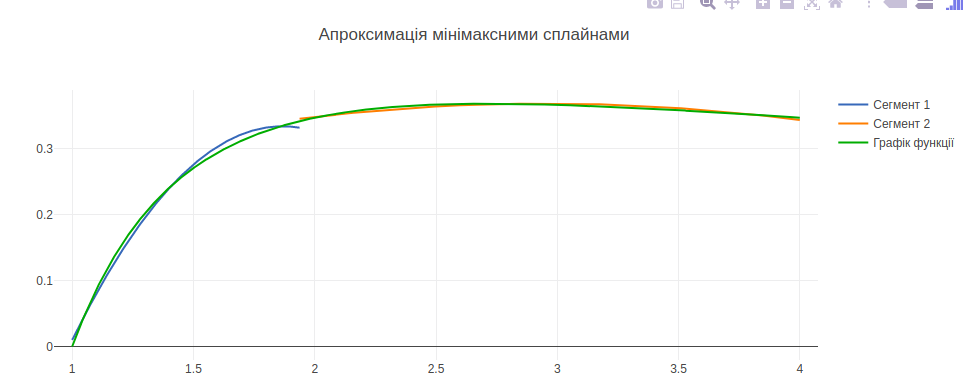
\includegraphics[scale=0.5]{example1}
% 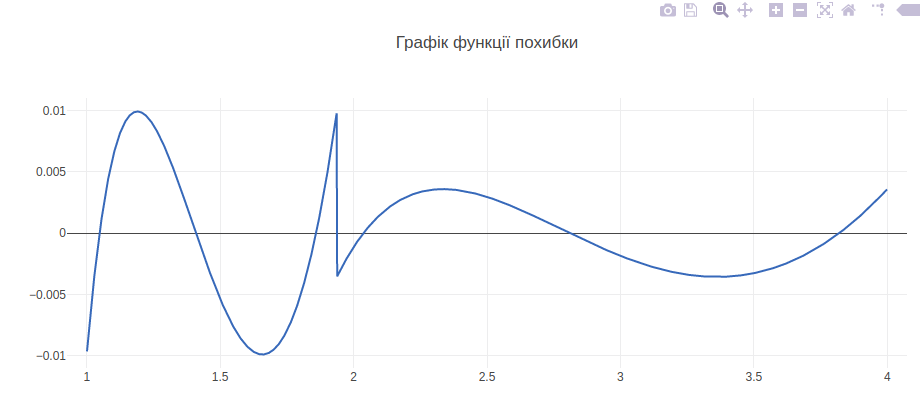
\includegraphics[scale=0.5]{example1_error} \\
% 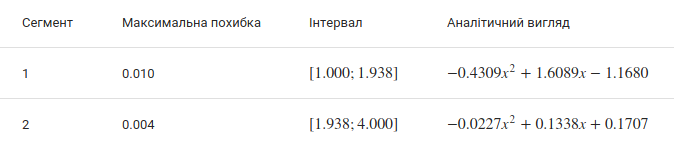
\includegraphics[scale=0.5]{example1_table}

% \newpage
% \textbf{Приклад 2}
% Вхідні дані:
% \vspace{0.5cm}
% \\
% 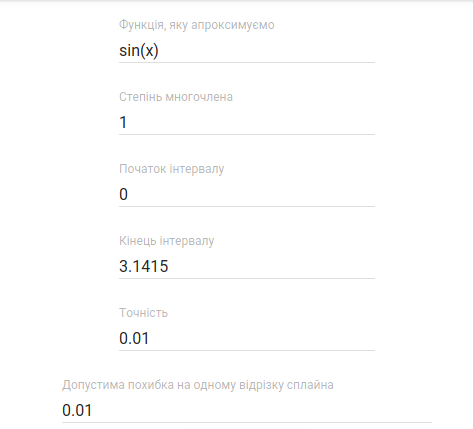
\includegraphics[scale=0.7]{example_2_inputs}

% \vspace{1cm}

% Результат роботи програми:
% \vspace{0.5cm}

% 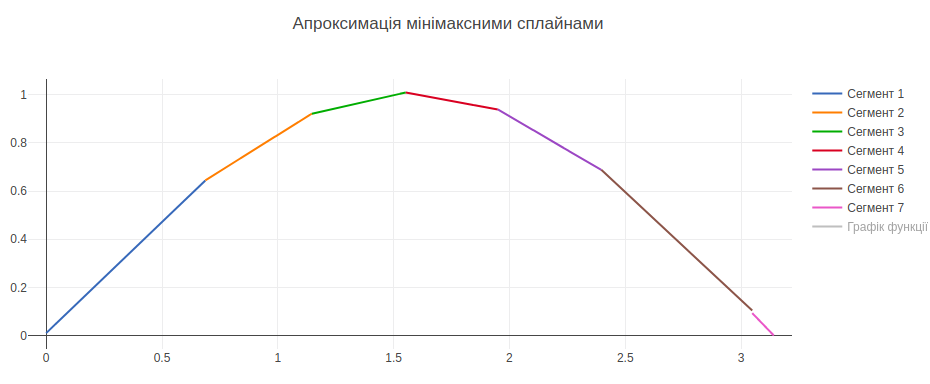
\includegraphics[scale=0.5]{example2}
% 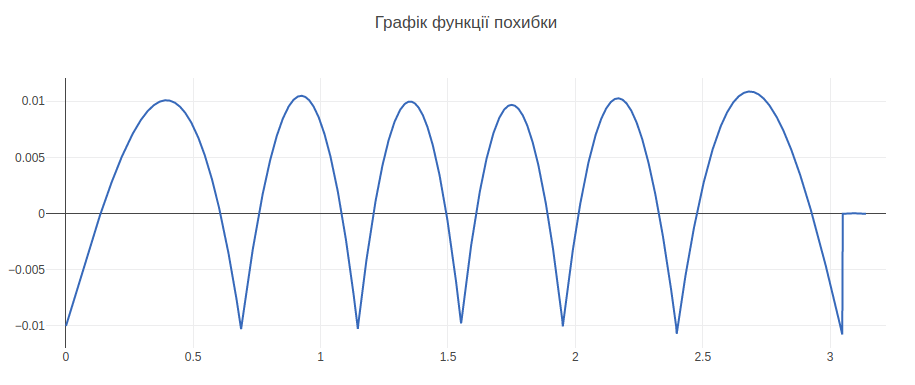
\includegraphics[scale=0.5]{example_2_error} \\
% \vspace{0.5cm}

% 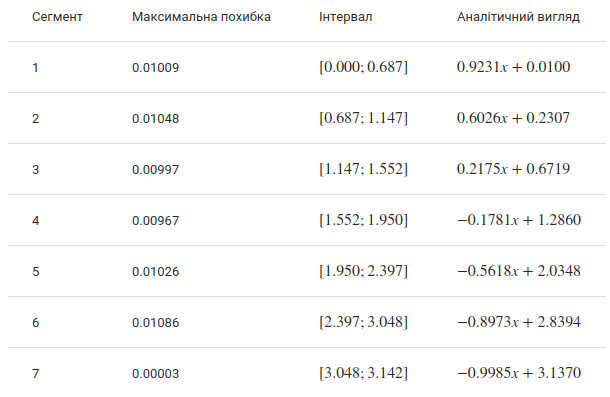
\includegraphics[scale=0.7]{example2_table}

% \newpage

% \textbf{Приклад 3}
% Вхідні дані:
% \vspace{0.5cm}
% \\
% 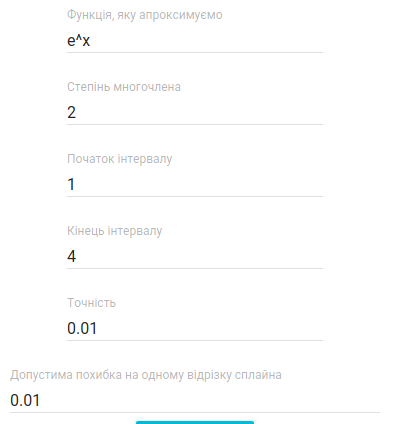
\includegraphics[scale=0.7]{example3_inputs}

% \vspace{1cm}

% Результат роботи програми:
% \vspace{0.5cm}

% 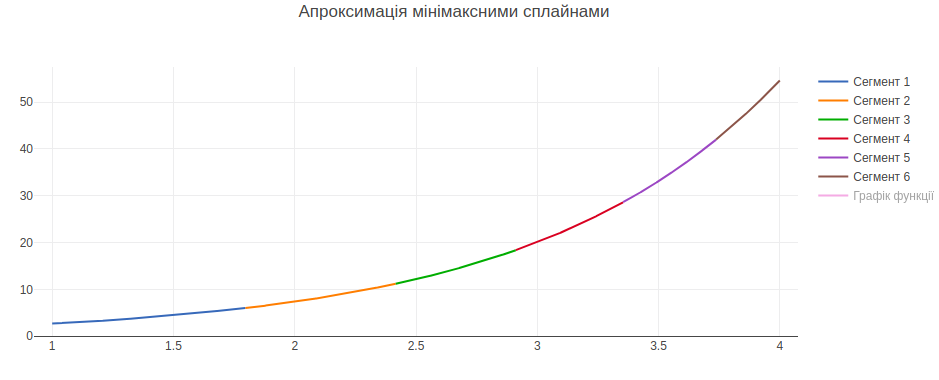
\includegraphics[scale=0.5]{example3}
% 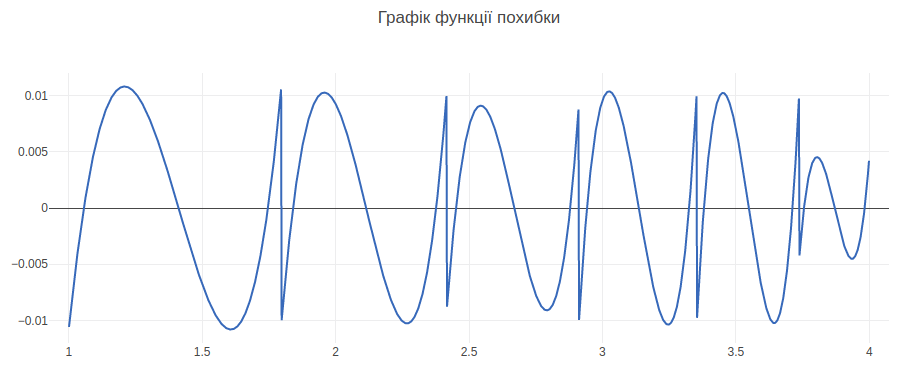
\includegraphics[scale=0.5]{example_3_error} \\
% \vspace{0.5cm}

% 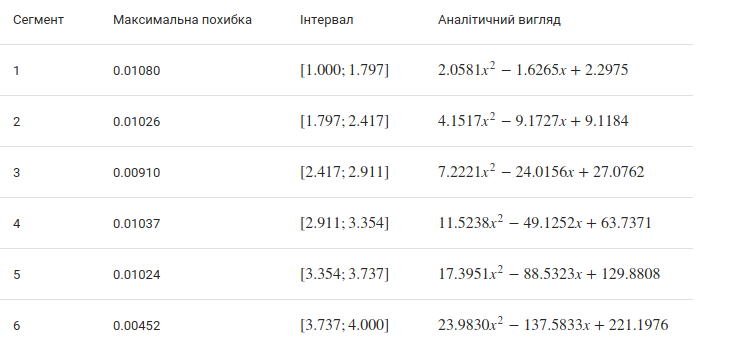
\includegraphics[scale=0.7]{example3_table}

% \newpage

% \textbf{Приклад 4 (Нерозривний сплайн)}
% Вхідні дані:
% \vspace{0.5cm}
% \\
% 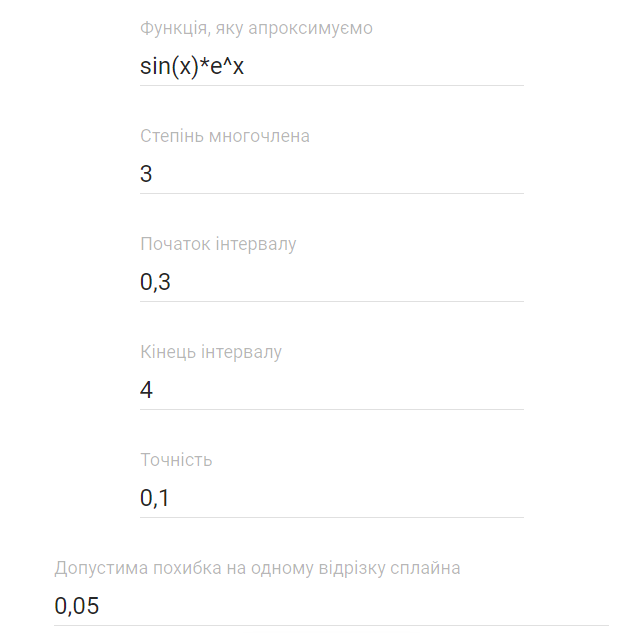
\includegraphics[scale=0.7]{example_4_inputs}

% \vspace{0.5cm}

% Результат роботи програми:

% \vspace{0.5cm}
% 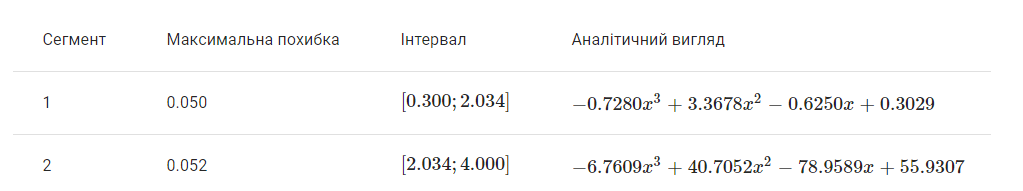
\includegraphics[scale=0.6]{example_4_table}

% 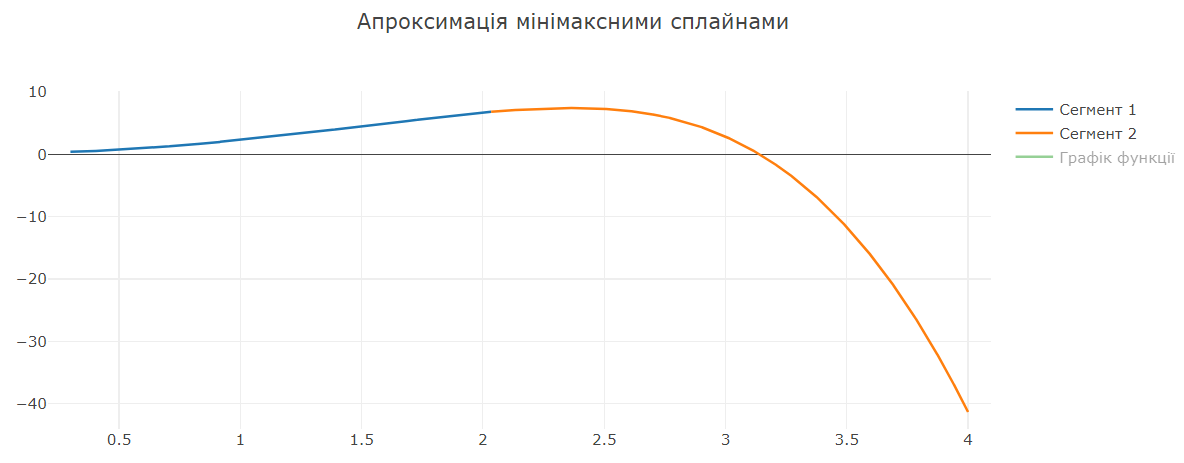
\includegraphics[scale=0.55]{example4}

% \vspace{1cm}

% 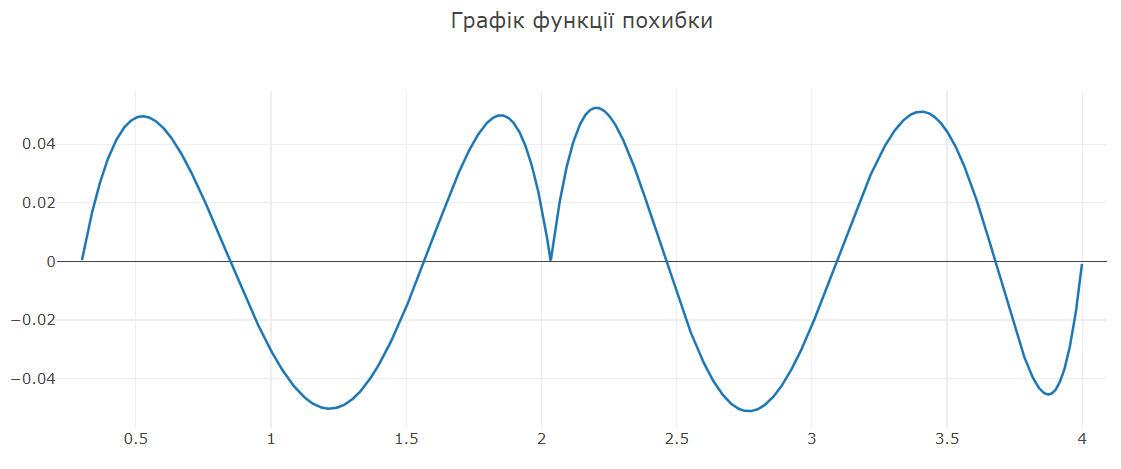
\includegraphics[scale=0.5]{example_4_error} 

\end{document}